\chapter{绪论}\label{chap:introduction}

本章将简要介绍本文研究主题的背景和意义。首先,本文会给出一些基础概念,这些概念在后续章节中会频繁使用,主要包括约束满足问题、AllDifferent约束以及其主要的求解算法,并引出研究该问题的动机。接着,本文会详细概述论文的主要工作内容。最后,本文将介绍论文的组织结构和框架。

\section{研究背景及意义}

% 开头,宏观
在当下信息时代,随着计算机科学和信息技术的飞速发展,约束满足问题(Constraint Satisfaction Problem,CSP)在各个领域中的应用也越来越广泛。无论是在工业生产、交通调度、金融决策,还是在人工智能、数据挖掘等高科技领域,我们都可以看到约束满足问题的身影。随着问题规模的增大和复杂度的提升,如何有效、高效地解决约束满足问题,已经成为了一个亟待解决的重要挑战。若未能及时有效地处理这些约束满足问题,可能会对相关领域的运作造成一定的影响。因此,研究一种高效求解约束满足问题的算法具有一定的理论意义和实践价值。

\subsection{约束满足问题}
% 介绍约束可满足问题。
约束满足问题是一类在各种领域中广泛应用的运筹学问题,它涉及到在一组特定的限制条件下,寻找一种满足所有约束的解决方案。在这类问题中,每一个约束都是对一组变量的取值范围的限制,只有当所有变量的取值都满足所有的约束时,我们才称这个赋值方案为一个解。求解约束满足问题的过程就是寻找这样的解的过程。约束满足问题的复杂性主要来自于两个方面:一方面,由于涉及的变量数量可能非常大,使得解空间的规模呈指数级增长;另外,由于约束的复杂性可能非常高,使得检查一个解是否满足所有约束的过程可能比较耗时。

% CSP的应用
约束满足问题在各个领域中都有广泛应用,其解决方案对于优化决策、提高效率等方面起着重要作用。约束满足问题在生产调度领域得到了广泛应用,它被用来优化生产流程和资源分配。例如,工厂在制定最优生产计划时,需要满足各种生产约束,如设备使用时间、原材料供应等,以此提高生产效率和降低成本。而在人工智能领域,约束满足问题则成为了实现自动推理、知识表示等核心任务的重要工具。智能机器人需要在满足物理规则、任务需求等环境约束的情况下,做出最优的决策和行动。此外,约束满足问题在网络安全领域也有重要应用,它被用于安全策略的制定和漏洞检测。网络管理员需要在满足权限控制、安全规则等安全约束的情况下,制定出最优的安全策略,以保护网络系统的安全。

% CSP的求解
为了有效解决约束满足问题,学术界和工业界已经提出和发展了许多不同类型的算法。这些算法大致可以分为两类:完备搜索算法\cite{van2006backtracking}和启发式搜索算法\cite{hoos2006local}。
完备搜索算法,如回溯搜索和深度优先搜索等,是最早被提出和使用的求解约束满足问题的算法。这类算法的主要思想是对解空间进行系统的遍历,直到找到一个满足所有约束的解,或者确定不存在这样的解为止。然而,由于约束满足问题的解空间通常非常大,这类算法在处理大规模问题时会面临严重的时间和空间复杂性问题。
因此,研究者们提出了启发式搜索算法,这类算法的主要思想是通过一些启发式的策略,如随机性、局部搜索等,来引导搜索过程,以期在较短的时间内找到满足约束的解,或者尽可能好的解。这类算法在处理大规模和复杂的约束满足问题时,表现出了较好的效果。
除了前述两种算法,神经网络的研究进展也引发了新的研究热点,也即利用神经方法解决约束满足问题。然而,尽管这种新方法在某些特定结构的问题上表现出色,但在泛化能力和求解准确率方面,仍然存在一定的局限性。
接下来,本文将重点介绍前两类算法的求解思路,并介绍算法涉及的各种求解策略。

% 求解CSP的完备搜索算法
完备搜索算法,也称为穷举搜索算法,完备搜索算法能够保证找到问题的所有解。最常见的完备搜索算法包括回溯搜索算法等。
回溯搜索算法是一种基于试错的策略,它在搜索过程中会记住已经访问过的状态,当发现当前的选择不能导致解的时候,就会撤销上一步的选择,回溯到前一状态,然后再进行选择。深度优先搜索算法则是一种基于堆栈的搜索策略,它总是对最新发现的状态进行扩展,直到找到解或者发现该状态无法扩展为止。
虽然完备搜索算法在理论上能够解决所有的约束满足问题,但是在实际应用中,由于解空间的规模通常非常大,导致完备搜索算法在处理大规模问题时面临严重的时间和空间复杂性问题。因此,目前主流的完备搜索算法都结合了约束传播\cite{bartak2001theory}、学习子句归结\cite{beame2003understanding}以及重启策略\cite{huang2007effect}等,进一步缩小搜索的范围和提高求解的效率。

% 求解CSP的局部搜索算法
局部搜索算法是求解约束满足问题的另一种重要方法。相比于完备搜索算法,局部搜索算法不再对所有可能的解进行遍历,而是从一个初始解出发,通过不断地在解的邻域中搜索,寻找满足约束的解,或者使得某种评价函数值更优的解。局部搜索算法的主要优点是能够在较短的时间内找到满足约束的解或者较优的解,特别是在处理大规模问题时,局部搜索算法通常能够提供更高的效率。然而,局部搜索算法也存在一些缺点,例如可能陷入局部最优解,或者在解空间中的搜索过程缺乏方向性等。同时,局部搜索算法一般是不完备的,也即无法判断问题是否是不可满足的(无解)。
常见的局部搜索算法包括模拟退火\cite{van1987simulated}、遗传算法\cite{mirjalili2019genetic}、粒子群算法\cite{wang2018particle}等算法。这些算法都通过引入一定的随机性和启发性,以期在全局范围内寻找到更优的解。例如,模拟退火算法模拟物理退火过程中的随机搜索,遗传算法则模拟自然界中的进化过程进行搜索。
在实际应用中,人们通常会根据问题的特性和需求,选择合适的局部搜索算法,或者将多种算法进行组合,以期得到更好的求解效果。

% 求解CSP的其他算法
除了完备搜索算法和局部搜索算法外,还可以将约束满足问题转换为其他类型的问题,如布尔可满足性问题(SAT)\cite{biere2009handbook}、可满足性模理论问题(SMT)\cite{barrett2018satisfiability}或整数线性规划问题(ILP)\cite{dantzig2002linear},然后使用相应的求解器来求解。其中,布尔可满足性问题是计算机科学中最基本的决策问题之一,通过将CSP中的每个变量和约束用多个布尔变量和布尔逻辑公式编码,可以将离散的CSP问题转化为SAT问题,并可以利用MiniSAT\cite{sorensson2005minisat}、Kissat等成熟的SAT求解器对其求解。SMT问题在SAT问题的基础上,进一步引入了一些理论和谓词约束,从而能够编码更高阶的逻辑问题。通过将CSP约束转化为函数,可以轻松的将CSP转化为SMT问题,并利用SMT求解器(如Z3\cite{de2008z3}、CVC5\cite{barbosa2022cvc5}等)来求解。LP问题是一种优化问题,CSP问题也可以视为一类有界的整数规划问题,因此可以利用CPLEX、Gurobi等线性规划求解器对其求解。这些方法的主要优点是能够利用已有的成熟工具和算法,将CSP问题的求解转化为已知问题的求解,从而提高求解的稳定性。然而,这些方法也存在一些局限性,例如转换过程可能会引入额外的复杂性,或者可能无法完备保留原问题的所有信息等。

% AllDifferent约束及其应用
\subsection{AllDifferent约束}
AllDifferent约束\cite{van2001alldifferent}是CSP中的一种常见的全局约束,它要求一组变量的取值都不相同。这种约束在很多实际问题中都有应用,例如在数独游戏中,要求每行、每列和每个子宫格内的数字都必须不同,这种限制就可以用AllDifferent约束来表示。通常,AllDifferent约束还常常与其他类型的约束(如线性约束、区间约束等)结合使用,以描述更复杂的问题。
由于AllDifferent约束要求所有变量的取值都必须不同,因此在搜索过程中,一旦有两个变量被赋予了相同的值,就可以立即判定当前的部分解不可行,从而避免无效的搜索。

在许多实际应用中,可以见到AllDifferent约束的影子。例如,在处理排班问题时,可以利用AllDifferent约束来保证在一个特定的时间段内,每个员工的工作任务都是独一无二的,这样就能避免任务冲突。而对于车辆路径问题,该约束可以帮助确保每辆车的行驶路径都是各不相同的,这样就能更好地优化路线,减少交通拥堵的可能性。
另一方面,Alldifferent约束可以建模许多经典的CSPs,例如数独、拉丁方、正交拉丁方、N皇后和全间隔问题等。这些问题有着广泛的应用,例如光网络\cite{kumar1999approximating},纠错码\cite{colbourn2004permutation},以及空中交通管理\cite{barnier2004graph}等。此外,拉丁方以及其变体正交拉丁方在组合测试上也有应用\cite{mandl1985orthogonal, zhang2014automatic}。

% AllDifferent约束的过滤算法和启发式算法
针对AllDifferent约束的求解,主流的方法是采用过滤算法对约束进行化简,之后再通过搜索和约束传播得到满足约束的赋值。最主流的过滤算法是基于匹配的过滤算法\cite{regin1994filtering}。这种算法将AllDifferent约束转化为一个二分图匹配问题:每个变量对应图的一个节点,每个可能的取值也对应一个节点,如果一个变量可以取某个值,则在对应的两个节点之间连一条边。然后,寻找这个图的一个完全匹配,即找到一种方式,使得每个变量节点都与一个取值节点相连,并且所有的边都不相交。如果找不到这样的完全匹配,那么原问题就无解。在实际操作中,通常使用网络流算法(如Ford-Fulkerson算法\cite{ford1957simple}或Edmonds-Karp算法\cite{edmonds1972theoretical})来寻找完全匹配。目前关于AllDifferent约束的优化思路大多基于此类思想,通过减少或避免匹配的复杂度或者复用匹配过程的信息来优化化简的时间。此外,针对AllDifferent约束,还存在一些启发式的策略\cite{michel2002constraint},该策略通过为部分约束涉及的变量赋不同的值,将这些约束视为隐含约束,从而只针对其他约束进行求解,之后再通过交换AllDifferent约束中变量的赋值来寻找整个问题的可行解。

% 当前求解的难点
虽然已有的求解AllDifferent约束的算法在很多情况下都能够工作得很好,但是它们仍然存在一些局限性和挑战。
对于大规模的问题,过滤算法可能会遇到效率问题。尽管过滤算法可以有效地剪枝搜索空间,但是在问题规模较大的情况下,过滤过程本身的计算量也可能会变得非常大。特别是当使用基于匹配的过滤算法时,需要解决的二分图匹配问题的规模可能会非常大,导致求解时间过长。
启发式策略的性能同样受到问题规模和约束难度的影响,在问题规模变大或约束结构复杂时,无法同时保证多个隐含约束,从而导致算法的性能下降严重。
最后,对于一些特殊的AllDifferent约束,例如包含了额外的条件或限制的AllDifferent约束,现有的算法可能无法直接应用,针对一类问题设计的策略可能无法泛化到更广的范围上去,需要进行额外的处理或修改,这同样增加了算法设计和实现的复杂性。
因此,如何进一步提高算法的效率和通用性,仍然是一个重要的研究方向。

\section{论文主要工作}

本文重点关注的是包含AllDifferent约束的约束满足问题。本文的目标是研究如何利用AllDifferent约束的特性,从而设计高效求解此类问题的局部搜索算法。本文特别关注那些大规模的、困难的样例,因为这些样例在实际应用中很常见,但对现有的算法来说,求解这些样例往往是最具挑战性的。

本文考虑在几类具有代表性的问题上进行实验,期望取得超越目前已有的启发式算法和主流约束规划算法的效果。
具体地,本文将数独\cite{simonis2005sudoku}、N皇后\cite{rivin1994n}、全间隔\cite{morris1974structure}、正交拉丁方问题\cite{mann1942construction}使用AllDifferent约束进行了建模,并通过研究这几类问题的特点,设计一个较为完善的针对此类问题的求解算法。
在算法部分,本文主要考虑以下几个方面:
\begin{itemize}
% \renewcommand{\labelenumi}{\theenumi)}
    \item 考虑如何将问题转化为便于采用局部搜索算法的形式,并进行化简;
    \item 设计用于局部搜索算法的操作算子和代价函数,构造局部搜索框架;
    \item 设计针对性的补充策略,如禁忌策略、打破平局策略和重启策略等。
\end{itemize}

对此,本文设计了用于解决包含AllDifferent约束的约束满足问题的局部搜索算法,其整体过程如图\ref{fig:total}所示。此外,本文根据该算法开发了相应的求解工具,并通过实验展示了其高效的求解能力。

其中,本文将在图上的操作定义为修改一个变量的赋值,同时一个操作的代价函数定义为修改前后图中存在冲突的边的个数。
这意味着可以将选择操作的步骤分为两步:首先选择变量,然后选择值。同时,可以相应地为每一步设计一个新的代价函数,即变量当前赋值导致的冲突边的个数和改变赋值后导致的冲突边的个数(这两者相减即操作的代价函数)。
在定义完局部搜索中最关键的两个概念后,算法的整体框架基本就可以得到了。此外,仍然需要设计一些新的策略来保证算法更少地陷入循环和局部最优解,这是局部搜索算法常见的两个挑战。
补充的策略可分为禁忌策略、打破平局策略和重启策略三个部分:在禁忌策略中,为操作的两个步骤分别设计了禁忌策略和性能检测器;在打破平局策略中,本文设计了新的细粒度的打分函数;在重启策略中,会根据迭代得到的当前解,来动态地调整下一次迭代的打分准则和迭代次数等参数。

具体的,本文介绍的工作主要包含三个方面的贡献:
\begin{itemize}
% \renewcommand{\labelenumi}{\theenumi)}
    \item 首先,本文将约束满足问题用图进行表示,这是局部搜索擅长求解的问题类型。与以往的策略不同,本文并不会对每个AllDifferent约束建图,而是将它们组合在一起,通过提取变量、表达式之间的关系,用一张图表示整个问题。这样得到的异构图有利于设计局部搜索需要定义的状态、操作等术语,也便于提出更高效的弧一致性算法。
    \item 其次,本文将根据得到的异构图,设计合适的移动操作(它同时定义了邻域)和打分函数,构造了针对问题求解的局部搜索的整体框架。通过引入其他针对问题特征的优化策略,如重启策略、禁忌策略等,可以保证算法的高效性,这些策略也具有一定的通用性,为局部搜索求解提供了新的思路。
    \item 最后,本文根据前面提到的求解算法AllDiff-LS设计了针对包含AllDifferent约束的CSP的求解工具,它可以在很短的时间内解决几乎所有问题。通过一系列比较实验,本文证明了算法的有效性,其求解效果在问题规模较小和较大的CSP上都极具竞争力,超越了找到的已知求解器。此外,本文通过消融实验也证明了算法的各个策略的有效性,这些策略结合在一起保证了算法的高效性。
\end{itemize}

\begin{figure*}[]
    \centering
    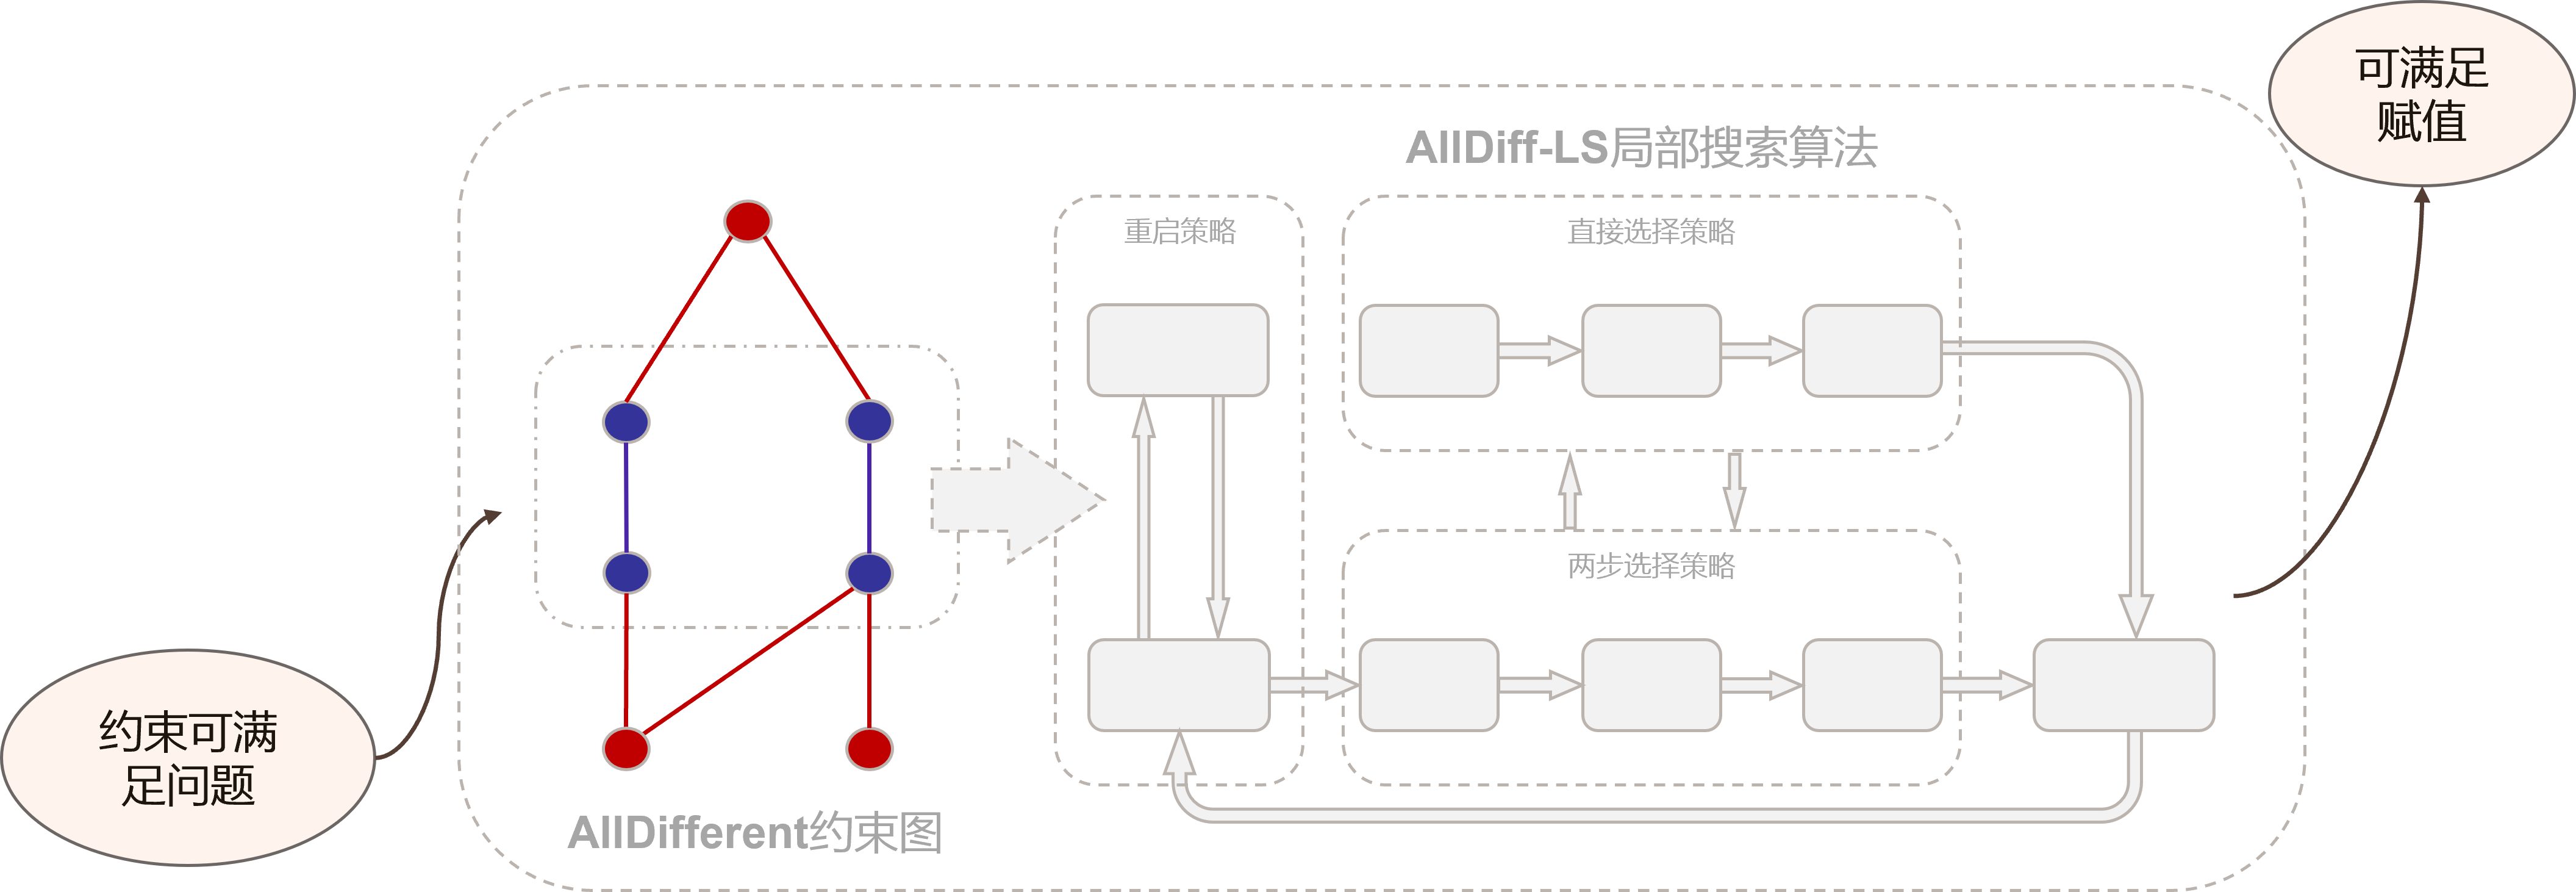
\includegraphics[width=0.9\columnwidth]{Img/all.png}
    \bicaption {工作的整体框架。} {The overall framework of the work.}
    \label{fig:total}
\end{figure*}

\section{论文组织}

本文的后续章节按照以下方式组织:

第二章:介绍本文所涉及的相关技术及研究现状。

第三章:介绍本文关于AllDifferent约束求解算法的设计思路及实现过程。

第四章:介绍基于第三章算法设计的加权和重启策略。

第五章:介绍本文在实验评估阶段的实验设计及结果分析。

第六章:总结了本文的主要贡献并展望了进一步的研究工作。